\documentclass[letta4 paper]{article}
% Set target color model to RGB
\usepackage[inner=2.0cm,outer=2.0cm,top=2.5cm,bottom=2.5cm]{geometry}
\usepackage{setspace}
\usepackage[rgb]{xcolor}
\usepackage{verbatim}
\usepackage{subcaption}
\usepackage{amsgen,amsmath,amstext,amsbsy,amsopn,tikz,amssymb,tkz-linknodes}
\usepackage{fancyhdr}
\usepackage[colorlinks=true, urlcolor=blue,  linkcolor=blue, citecolor=blue]{hyperref}
\usepackage[colorinlistoftodos]{todonotes}
\usepackage{rotating}
\usepackage{listings}
\lstset{
%	language=bash,
	basicstyle=\ttfamily
}

\newcommand{\ra}[1]{\renewcommand{\arraystretch}{#1}}

\newtheorem{thm}{Theorem}[section]
\newtheorem{prop}[thm]{Proposition}
\newtheorem{lem}[thm]{Lemma}
\newtheorem{cor}[thm]{Corollary}
\newtheorem{defn}[thm]{Definition}
\newtheorem{rem}[thm]{Remark}
\numberwithin{equation}{section}
\graphicspath{ {./img/} }

\newcommand{\homework}[6]{
   \pagestyle{myheadings}
   \thispagestyle{plain}
   \newpage
   \setcounter{page}{1}
   \noindent
   \begin{center}
   \framebox{
      \vbox{\vspace{2mm}
    \hbox to 6.28in { {\bf F1TENTH Autonomous Racing \hfill {\small (#2)}} }
       \vspace{6mm}
       \hbox to 6.28in { {\Large \hfill #1  \hfill} }
       \vspace{6mm}
       \hbox to 6.28in { {\it Instructor: {\rm #3} \hfill Name: {\rm #5}, StudentID: {\rm #6}} }
       %\hbox to 6.28in { {\it T\textbf{A:} #4  \hfill #6}}
      \vspace{2mm}}
   }
   \end{center}
   \markboth{#5 -- #1}{#5 -- #1}
   \vspace*{4mm}
}


\newcommand{\problem}[3]{~\\\fbox{\textbf{Problem #1: #2}}\hfill (#3 points)\newline}
\newcommand{\subproblem}[1]{~\newline\textbf{(#1)}}
\newcommand{\D}{\mathcal{D}}
\newcommand{\Hy}{\mathcal{H}}
\newcommand{\VS}{\textrm{VS}}
\newcommand{\solution}{~\newline\textbf{\textit{(Solution)}} }

\newcommand{\bbF}{\mathbb{F}}
\newcommand{\bbX}{\mathbb{X}}
\newcommand{\bI}{\mathbf{I}}
\newcommand{\bX}{\mathbf{X}}
\newcommand{\bY}{\mathbf{Y}}
\newcommand{\bepsilon}{\boldsymbol{\epsilon}}
\newcommand{\balpha}{\boldsymbol{\alpha}}
\newcommand{\bbeta}{\boldsymbol{\beta}}
\newcommand{\0}{\mathbf{0}}


\usepackage{booktabs}



\begin{document}

	\homework {Lab 3: Wall Following}{Due Date:}{INSTRUCTOR}{}{STUDENT NAME}{ID}
	\thispagestyle{empty}
	% -------- DO NOT REMOVE THIS LICENSE PARAGRAPH	----------------%
	\begin{table}[h]
		\begin{tabular}{l p{14cm}}
		\raisebox{-2cm}{
\includegraphics[scale=0.5, height=2.5cm]{f1_stickers_02} } & \textit{This lab and all related course material on \href{http://f1tenth.org/}{F1TENTH Autonomous Racing} has been developed by the Safe Autonomous Systems Lab at the University of Pennsylvania (Dr. Rahul Mangharam). It is licensed under a \href{https://creativecommons.org/licenses/by-nc-sa/4.0/}{Creative Commons Attribution-NonCommercial-ShareAlike 4.0 International License.} You may download, use, and modify the material, but must give attribution appropriately. Best practices can be found \href{https://wiki.creativecommons.org/wiki/best_practices_for_attribution}{here}.}
		\end{tabular}
	\end{table}
	% -------- DO NOT REMOVE THIS LICENSE PARAGRAPH	----------------%
	
	\noindent \large{\textbf{Course Policy:}} Read all the instructions below carefully before you start working on the assignment, and before you make a submission. All sources of material must be cited. The University Academic Code of Conduct will be strictly enforced.
	
	\section{Learning outcomes}

	The goal of this lab is to ...
		
	\begin{itemize}
		\item PID Controllers
		\item Driving the car autonomously via Wall Following
	\end{itemize}
	
	\section{Review of PID in the time domain}
	In the lecture we saw PID in the frequency domain, since that brings out most clearly the effects of the various gains and why we might want to add, say, a derivative term.
	Here we look at PID in the time domain, in relation to the task of wall-following.
	
	A PID controller is a way to maintain certain parameters of a system around a specified set point. PID controllers are used in a variety of applications requiring closed-loop control, such as in the VESC speed controller on your car.
	
	The general equation for a PID controller in the time domain, as discussed in lecture, is as follows:
	
	\begin{equation*}
	u(t) = K_{p} \; e(t) + K_{i}\; \int_{0}^{t}e(t^{\prime}) \; dt^{\prime} + K_{d}\; \frac{d}{dt}(e(t))
	\end{equation*}
	
	Here, $K_p$, $K_i$, and $K_d$ are constants that determine how much weight each of the three components (proportional, integral, derivative) contribute to the control output $u(t)$. $u(t)$ in our case is the steering angle we want the car to drive at. The error term $e(t)$ is the difference between the set point and the parameter we want to maintain around that set point.
	
	\section{Wall Following}
	
	In the context of our car, the desired distance to the wall should be our set point for our controller, which means our error is the difference between the desired and actual distance to the wall. This raises an important question: how do we measure the distance to the wall, and at what point in time? One option would simply be to consider the distance to the right wall at the current time $t$ (let's call it $D_t$). Let's consider a generic orientation of the car with respect to the right wall and suppose the angle between the car's $x$-axis and the wall is denoted by $\alpha$. We will obtain two laser scans (distances) to the wall: one at an angle $\theta$ ($0 < \theta \leq 70$ degrees), and another at an angle of 0 degrees relative to the car's x-axis. Suppose these two laser scans return distances $a$ and $b$, respectively.\\
	
	\begin{center}
		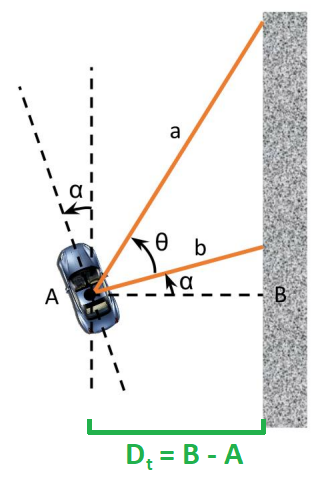
\includegraphics[scale=0.75]{wall_following_lab_figure_1.png}\\
		\label{fig:fig1}
		Figure 1: Distance and orientation of the car relative to the wall
	\end{center}
	
	Using the two distances $a$ and $b$ from the laser scan, the angle $\theta$ between the laser scans, and some trigonometry, we can express $\alpha$ as
	
	\begin{equation}
	\label{eq:alpha}
	\alpha = \mbox{tan}^{-1}\left(\frac{a \; \mbox{cos}(\theta) - b}{a \; \mbox{sin}(\theta)}\right)
	\end{equation}
	
	We can then express $D_t$ as 
	\begin{equation*}
	D_t = b \; \mbox{cos}(\alpha)
	\end{equation*}
	to get the current distance between the car and the right wall. What's our error term $e(t)$, then? It's simply the difference between the desired distance and actual distance! For example, if our desired distance is 1 meter from the wall, then $e(t)$ becomes $1 - D_t$.\\
	
	However, we have a problem on our hands. Remember that this is a race: your car will be traveling at a high speed and therefore will have a non-instantaneous response to whatever speed and servo control you give to it. If we simply use the current distance to the wall, we might end up turning too late, and the car may crash. Therefore, we must look to the future and project the car ahead by a certain lookahead distance (let's call it $L$). Our new distance $D_{t+1}$ will then be
	\begin{equation*}
	D_{t+1} = D_t + L \; \mbox{sin}(\alpha)
	\end{equation*}
	
	\begin{center}
		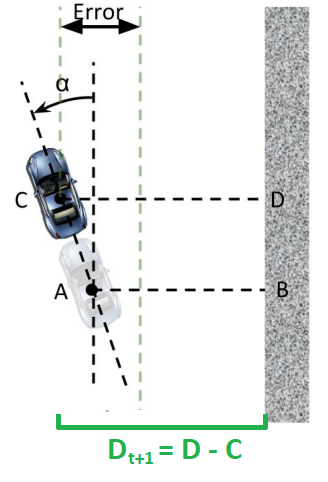
\includegraphics[scale=0.75]{wall_following_lab_figure_2.png}\\
		\label{fig:fig2}
		Figure 2: Finding the future distance from the car to the wall
	\end{center}
	
	We're almost there. Our control algorithm gives us a steering angle for the VESC, but we would also like to slow the car down around corners for safety. We can compute the speed in a step-like fashion based on the steering angle so that as the angle exceeds progressively larger amounts, the speed is cut in discrete increments. For this lab, we would like you to implement the following speed control algorithm:
	\begin{itemize}
		\item If the steering angle is between 0 degrees and 10 degrees, the car should drive at 1.5 meters per second.
		\item If the steering angle is between 10 degrees and 20 degrees, the speed should be 1.0 meters per second.
		\item Otherwise, the speed should be 0.5 meters per second.
	\end{itemize}
	
	So, in summary, here's what we need to do:
	\begin{enumerate}
		\item Obtain two laser scans (distances) $a$ and $b$, with $b$ taken at 0 degrees and $a$ taken at an angle $\theta$ ($0 < \theta \leq 70$)
		\item Use the distances $a$ and $b$ to calculate the angle $\alpha$ between the car's $x$-axis and the right wall.
		\item Use $\alpha$ to find the current distance $D_t$ to the car, and then $\alpha$ and $D_t$ to find the estimated future distance $D_{t+1}$ to the wall.
		\item Run $D_{t+1}$ through the PID algorithm described above to get a steering angle.
		\item Use the steering angle you computed in the previous step to compute a safe driving speed.
		\item Publish the steering angle and driving speed to the VESC.
	\end{enumerate}


	\section{Implementation}
	Implement left-wall following to make the car drive autonomously around the Levine Hall map. You can implement this node in either C++ or Python but the skeleton code is only in Python. You can download it from \href{https://github.com/f1tenth/f110\_ros}{https://github.com/f1tenth/f110\_ros}. You will only have to edit \texttt{wall\_follow.py}

	

	\section{Deliverables and Submission}
	% Make sure to place "labx" below with the correct lab number
	Submit the following as \texttt{studentname\_lab3.zip} (replace studentname with your name):
	
	\begin{enumerate}
		\item Your package named \texttt{studentname\_wallfollow.zip} including the wall following node. \textbf{Make sure it compiles before you submit after changing the package name.}
		\item Make a youtube video of wall following around the Levine Loop in the simulator add this link to a text file named \texttt{studentname\_lab3\_video.txt}
	\end{enumerate}

	\section{Grading}

	\subsection{Rubric}
	\begin{table}[h]
		\begin{tabular}{ll}
			\textbf{Topics} & \textbf{Points} \\
			Compilation & 10 \\
			Implemented PID & 40 \\
			Tuned PID & 40 \\
			Video & 10 \\
			\textbf{Total} & 100 \\
		\end{tabular}
	\end{table}
	

	
			
\end{document} 
